% =====================================================================
% Project R: conference paper draft (IEEE two-column conference format)
% Target venue: to be confirmed (QPAIN 2027, deadline 20 Dec 2026, and/or
% CVsports @ CVPR 2027). Page limit assumed 6 pages + references.
%
% Everything in \todo{...} (red) is a placeholder or an experiment we still
% have to run. Do NOT submit with any \todo left. Numbers that are NOT in a
% \todo come from runs on test1.mp4 already reported in Biweekly Report 3.
% =====================================================================
\documentclass[conference]{IEEEtran}
\IEEEoverridecommandlockouts

\usepackage{cite}
\usepackage{amsmath,amssymb,amsfonts}
\usepackage{graphicx}
\usepackage{textcomp}
\usepackage{xcolor}
\usepackage{booktabs}
\usepackage{multirow}
\usepackage{url}
\usepackage{tikz}
\usetikzlibrary{positioning,arrows.meta,fit,backgrounds}

\newcommand{\todo}[1]{\textcolor{red}{[TODO: #1]}}
\newcommand{\tbd}{\textcolor{red}{--}}

\begin{document}

\title{Translation-Free Real-Time Bengali Football Commentary from Broadcast Video with Identity-Grounded Templates}

\author{
\IEEEauthorblockN{Anik Mondal, Zuhayer Anjum Aryan, and Nabil Bin Hannan}
\IEEEauthorblockA{Department of Electrical and Computer Engineering, North South University, Dhaka, Bangladesh\\
\{anik.mondal01, anjum.aryan\}@northsouth.edu, \todo{supervisor email}}
}

\maketitle

% ---------------------------------------------------------------------
\begin{abstract}
Automatic sports commentary research has focused almost entirely on English, and the usual route to a low-resource language, generating English text with a large language model and then translating it, adds latency and can corrupt player names. We present a pipeline that turns single-camera broadcast football video into spoken Bengali commentary without any translation step. A perception stage detects and tracks players, keeps a stable identity for each player across camera pans, occlusions and broadcast cuts, assigns players to teams, and recognises shirt names and numbers. An event stage fuses a learned action-spotting model with scoreboard reading and card detection, and links each event to the players involved. A generation stage fills hand-written Bengali templates for 30 event types, referring to each player by name, else shirt number, else shirt colour, and speaks the line with Bengali text-to-speech at the event's time. On a 2-minute broadcast highlights clip, the identity layer reduces 495 raw tracker identities to 259, and the fused event stage recovers all five annotated events (two goals, a corner, a foul and a red card), whereas the learned spotting model alone misses both goals and mislabels the card. \todo{Add SoccerNet tracking (HOTA/IDF1), spotting (mAP), and latency vs.\ an LLM+translation baseline once run.}
\end{abstract}

\begin{IEEEkeywords}
sports commentary generation, Bengali, multi-object tracking, action spotting, low-resource languages, football video analysis
\end{IEEEkeywords}

% ---------------------------------------------------------------------
\section{Introduction}

Bengali is spoken by more than 230 million people \todo{cite source for speaker count}, and football is among the most followed sports in Bangladesh and West Bengal, yet live Bengali commentary exists only for a handful of top matches. Local, school and amateur matches are filmed with a single camera but have no commentator at all. Automatic commentary could fill this gap, but existing systems generate English \cite{mkhallati2023soccernetcaption,qi2023goal,rao2024matchtime}, and adapting them to Bengali is not straightforward.

The common recipe for a low-resource language is to generate English text with a large language model (LLM) and translate it with a machine translation (MT) model such as NLLB \cite{nllb2022} or IndicTrans2 \cite{gala2023indictrans2}. For live commentary this has two costs. First, the two models run in sequence for every event, which adds latency to a task where a line is useless a few seconds late. Second, both models can change or invent player names: the LLM may hallucinate an entity that is not on the pitch, and MT may transliterate or translate a name inconsistently. In commentary, a wrong name is the most visible error a system can make.

We avoid both problems by never translating. Our system detects \emph{what} happened, \emph{when} and \emph{to whom} directly from the video, and fills hand-written Bengali templates whose slots (player, shirt number, minute) are grounded in that perception output. The quality of the commentary then depends on the perception stage, in particular on knowing which player is which over a whole broadcast. This is hard with a single moving broadcast camera: players leave and re-enter the view as the camera pans, are occluded by each other, and the broadcast cuts between wide shots, close-ups and replays, each of which makes a standard tracker issue new identities.

Our contributions are:
\begin{itemize}
\item An end-to-end, translation-free pipeline from broadcast football video to timed Bengali speech, built from open models and runnable on a single consumer GPU.
\item A stable player-identity layer on top of BoT-SORT \cite{aharon2022botsort} that compensates camera motion, detects shot cuts, re-links lost players by position and appearance, and corrects identity swaps between players of different teams.
\item A multi-source event stage that fuses learned action spotting \cite{giancola2021temporally} with scoreboard-based goal detection and image-based card detection, and links events to players.
\item A Bengali referring-expression fallback (name, else shirt number, else shirt colour) that keeps every template slot grounded in what was actually recognised, together with a Bengali template set covering 30 event types.
\item \todo{A preliminary evaluation on SoccerNet benchmarks and a latency comparison against an LLM+MT baseline.}
\end{itemize}

% ---------------------------------------------------------------------
\section{Related Work}

\textbf{Automatic sports commentary.} Early systems generated commentary from structured play data, for example live football text from event logs \cite{taniguchi2019generating}. Recent work generates commentary from video: SoccerNet-Caption introduced dense, timestamped commentary for football broadcasts \cite{mkhallati2023soccernetcaption}, GOAL added knowledge-grounded commentary with player and team information \cite{qi2023goal}, and MatchTime improved the alignment between video and commentary text and trained a video-language commentary model \cite{rao2024matchtime}. All of these produce English, and the end-to-end models often name players that are not in the scene. Our work targets Bengali and grounds every entity in perception output instead of generating it.

\textbf{Football video understanding.} SoccerNet provides large-scale benchmarks for action spotting \cite{deliege2021soccernet}, player tracking \cite{cioppa2022soccernet} and game-state reconstruction \cite{somers2024soccernetgsr}. Action spotting methods pool frame features over a temporal window, from NetVLAD-based pooling \cite{giancola2021temporally,arandjelovic2016netvlad} to end-to-end models \todo{cite E2E-Spot / T-DEED}. Multi-object trackers such as ByteTrack \cite{zhang2022bytetrack} and BoT-SORT \cite{aharon2022botsort} associate detections frame by frame but are not designed to keep identities across broadcast cuts. Jersey-number recognition has recently been built on scene-text recognisers such as PARSeq \cite{bautista2022scene,koshkina2024general}. We combine these components and add an identity layer and event fusion aimed at commentary.

\textbf{Bengali language technology.} Bengali NLP has progressed with pretrained models such as BanglaBERT \cite{bhattacharjee2022banglabert} and multilingual MT \cite{nllb2022,gala2023indictrans2}, and multilingual speech synthesis now covers Bengali \cite{pratap2024scaling}. To our knowledge, no prior work generates Bengali sports commentary from video. \todo{Verify with a literature search before submission.}

% ---------------------------------------------------------------------
\section{System Overview}

\begin{figure*}[t]
\centering
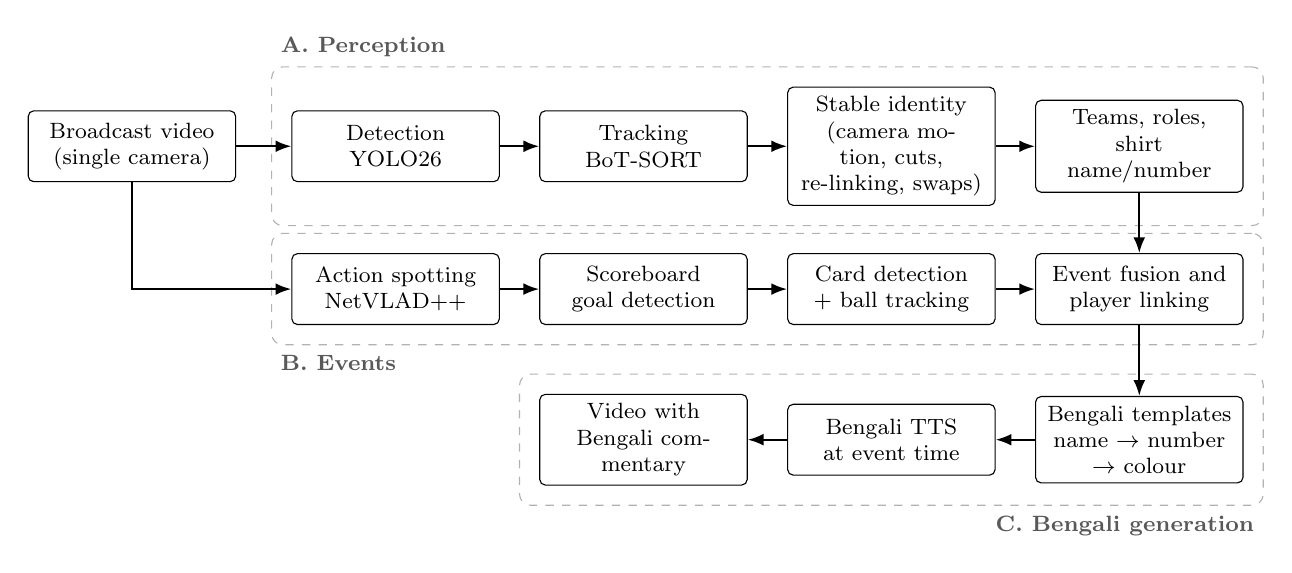
\begin{tikzpicture}[
  node distance=4mm and 5mm,
  box/.style={draw, rounded corners=2pt, align=center, font=\footnotesize, minimum height=9mm, text width=24mm, fill=white},
  stage/.style={draw=gray!60, dashed, rounded corners=4pt, inner sep=2.5mm},
  lbl/.style={font=\footnotesize\bfseries, text=gray!70!black},
  arr/.style={-{Latex[length=2mm]}, thick}
]
\node[box] (video) {Broadcast video\\(single camera)};
\node[box, right=7mm of video] (det) {Detection\\YOLO26};
\node[box, right=of det] (trk) {Tracking\\BoT-SORT};
\node[box, right=of trk] (id) {Stable identity\\(camera motion, cuts,\\re-linking, swaps)};
\node[box, right=of id] (team) {Teams, roles,\\shirt name/number};

\node[box, below=9mm of det] (spot) {Action spotting\\NetVLAD++};
\node[box, right=of spot] (score) {Scoreboard\\goal detection};
\node[box, right=of score] (card) {Card detection\\+ ball tracking};
\node[box, right=of card] (fuse) {Event fusion and\\player linking};

\node[box, below=9mm of fuse] (tmpl) {Bengali templates\\name $\rightarrow$ number\\$\rightarrow$ colour};
\node[box, left=of tmpl] (tts) {Bengali TTS\\at event time};
\node[box, left=of tts] (out) {Video with\\Bengali commentary};

\draw[arr] (video) -- (det);
\draw[arr] (det) -- (trk);
\draw[arr] (trk) -- (id);
\draw[arr] (id) -- (team);
\draw[arr] (video.south) |- (spot.west);
\draw[arr] (spot) -- (score);
\draw[arr] (score) -- (card);
\draw[arr] (card) -- (fuse);
\draw[arr] (team.south) -- (fuse.north -| team.south);
\draw[arr] (fuse) -- (tmpl);
\draw[arr] (tmpl) -- (tts);
\draw[arr] (tts) -- (out);

\begin{scope}[on background layer]
\node[stage, fit=(det)(trk)(id)(team)] (s1) {};
\node[stage, fit=(spot)(score)(card)(fuse)] (s2) {};
\node[stage, fit=(tmpl)(tts)(out)] (s3) {};
\end{scope}
\node[lbl, anchor=south west] at (s1.north west) {A. Perception};
\node[lbl, anchor=north west] at (s2.south west) {B. Events};
\node[lbl, anchor=north east] at (s3.south east) {C. Bengali generation};
\end{tikzpicture}
\caption{Overview of the pipeline. No stage generates or translates English text: Bengali templates are filled directly with entities recognised from the video.}
\label{fig:pipeline}
\end{figure*}

Fig.~\ref{fig:pipeline} shows the three stages. The perception stage (Section~\ref{sec:perception}) outputs, for every frame, the boxes of players, goalkeepers and the referee with a stable identity, team and, where readable, shirt name and number. The event stage (Section~\ref{sec:events}) outputs a list of timed events with the players involved. The generation stage (Section~\ref{sec:generation}) turns each event into a Bengali sentence and speech. The stages communicate through small structured files, so each can be evaluated and replaced on its own.

% ---------------------------------------------------------------------
\section{Perception}
\label{sec:perception}

\subsection{Detection and Tracking}
We detect people and the ball with YOLO26 \cite{jocher2026ultralyticsyolo26}. The COCO-pretrained model only knows ``person'' and ``sports ball'', so we fine-tune it on SoccerNet-Tracking \cite{cioppa2022soccernet} with four classes (player, goalkeeper, referee, ball), using only the training clips so that the official test clips remain unseen. \todo{Report detector mAP on the SoccerNet-Tracking test split, COCO vs.\ fine-tuned.} Detections are associated over time with BoT-SORT \cite{aharon2022botsort}. Boxes whose feet are not on grass (spectators, staff, faces in close-ups) and partial boxes contained in a larger box of the same player are removed.

\subsection{Stable Identity Layer}
BoT-SORT starts a new identity whenever it loses a player, which in broadcast video happens constantly. Our layer keeps its own identity for every player on top of the tracker's.

\textit{Camera motion.} For each frame we track background corners \cite{shi1994good} with pyramidal Lucas--Kanade flow \cite{lucas1981iterative}, excluding detected people, and fit a similarity transform with RANSAC \cite{fischler1981ransac}. Positions of players who left the view are warped by the accumulated transform, so a player who returns after a pan is expected where they actually are.

\textit{Shot cuts.} Cuts, dissolves and switches between two wide cameras are detected from abrupt changes in the colour histogram together with failed or implausible camera-motion estimates. Positions from before a cut are not trusted after it.

\textit{Re-linking.} A new tracker identity is held as pending for three frames and then matched to a currently missing player using a cost that combines predicted position (with a gate that grows with the time the player has been missing) and appearance. Appearance is a colour model of shirt and shorts and, optionally, an LMBN re-identification embedding \cite{herzog2021lightweight} trained on Market-1501 \cite{zheng2015scalable}. When only appearance is available (after a cut, or after more than about two seconds missing), a link is accepted only if it passes a stricter threshold and a ratio test against the second-best candidate; otherwise a new identity is issued, since a new identity is less harmful to commentary than a wrong one.

\textit{Identity swaps.} When two players cross, the tracker sometimes swaps their identities or moves one identity onto the other player. We (i) freeze a player's colour model while the observation disagrees with it, (ii) hand an identity back once two players of different kits separate and the identity clearly shows the other player, and (iii) release an identity whose player suddenly wears the other team's kit, using team colour models fitted online. Two teammates who swap cannot be separated by colour; this requires shirt numbers.

\subsection{Teams, Roles and Shirt Text}
Shirt and shorts colour descriptors are clustered into two teams with $k$-means \cite{lloyd1982least}, with each stable identity voting over all of its boxes. Identities that fit neither cluster are assigned by position: a goalkeeper is the last person at one end of play, the two goalkeepers always go to different teams, and the referee stays near the middle of play. With the fine-tuned detector, the detector's class decides the role directly.

Shirt names and numbers are read from torso crops with PARSeq \cite{bautista2022scene}, with text regions found by the CRAFT detector \cite{baek2019character}, restricting the output to digits or letters. A value is accepted only when at least two crops of the same identity agree. If a team roster is available, a number maps to a name and a misread name snaps to the closest roster entry.

% ---------------------------------------------------------------------
\section{Event Detection}
\label{sec:events}

\textit{Learned action spotting.} We run the official NetVLAD++ model \cite{giancola2021temporally} trained on SoccerNet-v2 \cite{deliege2021soccernet}. Frames are sampled at 2 fps and encoded with ResNet-152 \cite{he2016deep} exactly as in the SoccerNet features; the model scores 17 classes every 0.5\,s from a 15\,s window, and peaks after non-maximum suppression (10\,s window in our live setting) become events.

\textit{Scoreboard goals.} Broadcast highlights often cut the build-up and celebration that the spotting model relies on. We therefore locate the score graphic as the static region at the top of the frame, find its two score digits, and report a goal when one digit changes and stays changed for two seconds. The colours of the two halves of the graphic are matched to the team colours to decide which team scored.

\textit{Cards.} Yellow and red cards are detected as small, bright, saturated rectangles that stand alone in the frame with a person directly below, seen for about half a second, either above a tracked referee in wide shots or anywhere in close-ups. A card from the spotting model takes its colour and time from the card seen in the image.

\textit{Fusion and player linking.} The three sources are merged into one time-ordered list, with duplicate events within a short window removed and set pieces in the 20\,s after a goal (the kick-off) dropped. Ball candidates from the detector are filtered for temporal consistency after camera-motion compensation, and short gaps are interpolated. Ball possession then links each event to players: scorer and assist, fouler and fouled player, booked player and set-piece taker.

% ---------------------------------------------------------------------
\section{Bengali Commentary Generation}
\label{sec:generation}

\textit{Templates.} We wrote 83 Bengali commentary templates for 30 event types (goal, foul, yellow and red card, corner, free kick, goal kick, save, offside, penalty, and others), with slots for \texttt{\{player\}}, \texttt{\{jersey\}} and \texttt{\{minute\}}. \todo{Expand to the planned larger set and report counts per event type; describe who wrote and checked them.} Templates were written by native speakers in broadcast register rather than translated.

\textit{Referring-expression fallback.} Each player slot is filled with the most specific reliable description: the shirt name if read (or mapped from the roster), else ``the number $N$ shirt player'' in Bengali, else ``the \emph{colour}-shirt player'' using the team colour named in Bengali. Templates containing a \texttt{\{jersey\}} slot are used only when both name and number are known. This guarantees that every entity in the output was observed in the video.

\textit{Speech.} Lines are synthesised with Meta MMS-TTS for Bengali \cite{pratap2024scaling}, a VITS model \cite{kim2021conditional} that runs offline, or with neural Bengali voices from Edge TTS \cite{edge_tts_2024}. Each line is placed at its event's time, delayed only if the previous line is still playing, and mixed over the attenuated match audio.

% ---------------------------------------------------------------------
\section{Experiments}

\subsection{Data}
\textit{Case-study clip.} A 2-minute broadcast highlights clip of Manchester United vs.\ Tottenham (1280$\times$720, 25\,fps, 3{,}002 frames, 15 shot changes), with five events annotated by us: a corner, two goals, a foul and a red card.

\textit{Public benchmarks.} \todo{SoccerNet-Tracking test split (49 clips) for tracking; SoccerNet-v2 test split (100 matches) for spotting; SoccerNet jersey-number set for shirt reading. State exact splits.}

\textit{Full-match evaluation.} \todo{Our own labels (SoccerNet Labels-v2 format) on N full broadcast matches, needed for scoreboard and card detection, which need raw video.}

\subsection{Player Identity}
On the case-study clip, without ground truth, we count identities. BoT-SORT alone produces 495 identities; our layer reduces this to 259. In the first 18-second wide shot, the count falls from 47 to about 29, and identities that show both team colours for more than 20 frames fall from 15 to 5. Adding the LMBN embedding separates teammate pairs better than colour alone (AUC 0.85 vs.\ 0.79) but gives only a small gain on a 30\,s segment (cross-team identities 5 $\rightarrow$ 4).

\begin{table}[t]
\centering
\caption{Tracking on the SoccerNet-Tracking test split, with and without our identity layer. \todo{Run benchmarks/tracking\_benchmark.py.}}
\label{tab:tracking}
\begin{tabular}{llccc}
\toprule
Tracker & ID layer & HOTA $\uparrow$ & IDF1 $\uparrow$ & IDsw $\downarrow$ \\
\midrule
ByteTrack \cite{zhang2022bytetrack} & none & \tbd & \tbd & \tbd \\
ByteTrack & ours & \tbd & \tbd & \tbd \\
BoT-SORT \cite{aharon2022botsort} & none & \tbd & \tbd & \tbd \\
BoT-SORT & ours & \tbd & \tbd & \tbd \\
Deep OC-SORT & none & \tbd & \tbd & \tbd \\
Deep OC-SORT & ours & \tbd & \tbd & \tbd \\
\bottomrule
\end{tabular}
\end{table}

\todo{Note: SoccerNet-Tracking clips are 30\,s and contain no cuts, so they test occlusion and camera motion only; cut handling needs our own labelled broadcast clips.}

\subsection{Event Detection}

Table~\ref{tab:events} lists the events on the case-study clip. NetVLAD++ alone finds the corner and the foul, labels the red card as yellow, and misses both goals; the fused system recovers all five with correct types and times within \todo{x}\,s. Rule-based foul and free-kick detection, which we used before the learned model, produced only false positives on this clip, because highlights cut away before set pieces are taken.

\begin{table}[t]
\centering
\caption{Events on the case-study clip (video time).}
\label{tab:events}
\begin{tabular}{lll}
\toprule
Event & NetVLAD++ only & Fused (ours) \\
\midrule
Corner (0:53.5) & found & found \\
Goal 1--0 (1:02.8) & missed & found (scoreboard) \\
Foul (1:28.0) & found & found \\
Red card (1:35.1) & as yellow & found (card det.) \\
Goal 1--1 (1:49.6) & missed & found (scoreboard) \\
\bottomrule
\end{tabular}
\end{table}

\todo{Spotting on the SoccerNet-v2 test set: reproduce MaxPool, NetVLAD, CALF and NetVLAD++ average-mAP with benchmarks/spotting\_benchmark.py, check against published values, and report the cost of our 10\,s NMS. Report precision/recall/time error of the fused system on our full-match labels.}

\subsection{Shirt Reading}
On 417 per-player crop sets from the case-study clip, PARSeq with CRAFT reads a name or number for 29 players, against 13 for EasyOCR \cite{jaidedai_easyocr}, including names such as SOLANKE and TONALI. \todo{Accuracy on the SoccerNet jersey-number test set; how often each fallback level (name/number/colour) is used per event.}

\subsection{Latency and Commentary Quality}
\todo{Main experiment for the claim. Compare (a) ours: template filling, (b) English LLM (e.g.\ Llama~3 8B) then NLLB/IndicTrans2, (c) LLM prompted to write Bengali directly. Measure per-event latency from event time to start of speech on the same GPU, entity accuracy (wrong or invented player names), and human ratings (fluency, correctness, excitement) from $\geq$3 native speakers on $\geq$100 events.}

\begin{table}[t]
\centering
\caption{Per-event latency and entity errors. \todo{Run.}}
\label{tab:latency}
\begin{tabular}{lccc}
\toprule
Method & Text (ms) & To speech (ms) & Wrong names (\%) \\
\midrule
LLM $\rightarrow$ MT & \tbd & \tbd & \tbd \\
LLM direct Bengali & \tbd & \tbd & \tbd \\
Templates (ours) & \tbd & \tbd & \tbd \\
\bottomrule
\end{tabular}
\end{table}

\todo{End-to-end throughput (fps) of the whole pipeline on one GPU, per stage.}

% ---------------------------------------------------------------------
\section{Limitations}
Our quantitative results so far come from one highlights clip without frame-level ground truth, so identity counts are a proxy rather than accuracy. Teammates cannot yet be told apart reliably after a cut, ball detection with a general detector is weak, which limits scorer and fouler attribution, and scoreboard and card detection depend on broadcast graphics. Templates give correct but repetitive language. The pipeline currently processes recorded video; a streaming implementation is future work.

% ---------------------------------------------------------------------
\section{Conclusion}
We presented a translation-free pipeline that turns broadcast football video into spoken Bengali commentary, grounding every player reference in what the system recognises. A stable identity layer, multi-source event fusion and a name--number--colour fallback make this possible with open models on one GPU. Next we will evaluate each stage on SoccerNet and our own full-match labels, compare against LLM-plus-translation baselines on latency and entity accuracy, and extend the system to multiple cameras.

\section*{Acknowledgment}
\todo{Optional: thank NSU / CSE498R.}

\bibliographystyle{IEEEtran}
\bibliography{refs}

\end{document}
